\section{Příklad 3}
% Jako parametr zadejte skupinu (A-H)
\tretiZadani{E}

\large{\textbf{Řešení:}}

%%% Krok 1 - Úprava schémy
\begin{center}
    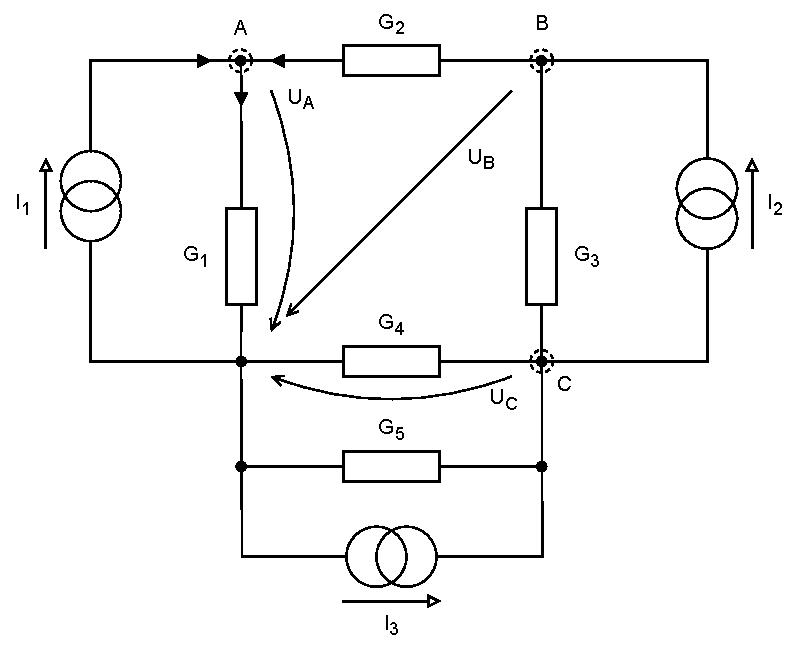
\includegraphics[scale=0.8,keepaspectratio]{fig/solutions/03-sol/03-step1.pdf} \\
    Obr.3.1 - Změníme zdroj napětí na zdroj proudu, označíme nezávislé uzly a vyznačíme si jednotlivé proudy, které vtekajou do uzlů
\end{center}

\noindent Převod odporu na vodivost a změna napětového zdroje na proudový
\begin{gather*}
    G = \frac{1}{R}\\\\
    I_3 = \frac{U}{R_5} = \frac{135}{21} = 6.42857143A
\end{gather*}
\\

%%% Krok 2 - Rovnice
Vytvořme rovnice pro jednotlivé uzly
\begin{gather*}
    A: U_A(-G_1 - G_2) + U_B(G_2) + U_C(0) = -I_1 \\\\
    B: U_A(G_2) + U_B(-G_2 - G_3) + U_C(G_3) = -I_2 \\\\
    C: U_A(0) + U_B(G_3) + U_C(-G_3 - G_4 - G_5) = I_2 - I_3
\end{gather*}

Převedeme do matice a vypočítáme pomocí Cramerova a Sarussova pravidla:
\begin{gather*}
    \begin{pmatrix}
        -G_1 -G_2 & G_2 & 0 \\
        G_2 & -G_2 - G_3 & G_3 \\
        0 & G_3 & -G_3 - G_4 - G_5
    \end{pmatrix}
    \times
    \begin{pmatrix}
        U_A \\
        U_B \\
        U_C
    \end{pmatrix}
    =
    \begin{pmatrix}
        -I_1 \\
        -I_2 \\
        I_2 - I_3
    \end{pmatrix}
\end{gather*}

\begin{gather*}
    \begin{pmatrix}
        - \frac{1}{52} - \frac{1}{42} & \frac{1}{42} & 0 \\
        \frac{1}{42} & - \frac{1}{42} - \frac{1}{52} & \frac{1}{52} \\
        0 & \frac{1}{52} & - \frac{1}{52} - \frac{1}{42} - \frac{1}{21}
    \end{pmatrix}
    \times
    \begin{pmatrix}
        U_A \\
        U_B \\
        U_C
    \end{pmatrix}
    =
    \begin{pmatrix}
        -0,55 \\
        -0,65 \\
        -5.77857143
    \end{pmatrix}
\end{gather*}

\begin{gather*}
    M = 
    \begin{vmatrix}
    - \frac{1}{52} - \frac{1}{42} & \frac{1}{42} & 0 \\
        \frac{1}{42} & - \frac{1}{42} - \frac{1}{52} & \frac{1}{52} \\
        0 & \frac{1}{52} & - \frac{1}{52} - \frac{1}{42} - \frac{1}{21}
    \end{vmatrix}
    = -0.00010063 \\\\
    M_{U_C} = 
    \begin{vmatrix}
        - \frac{1}{52} - \frac{1}{42} & \frac{1}{42} & -0,55 \\
        \frac{1}{42} & - \frac{1}{42} - \frac{1}{52} & -0,65 \\
        0 & \frac{1}{52} & -5.77857143
    \end{vmatrix}
    = -0.00821861
\end{gather*}
Po vypočítaní zjistíme, že:
\begin{gather*}
    U_C = \frac{M_{U_C}}{M} = \frac{-0.00821861}{-0.00010063} = 81.67000002 V
\end{gather*}
\\
Tímto způsobem můžeme vypočítat $\boldsymbol{U_{R_4}}$ a $\boldsymbol{I_{R_4}}$:
\begin{gather*}
    \boldsymbol{U_{R_4}} = U_C = \textbf{81.67000002V} \\
    \boldsymbol{I_{R_4}} = \frac{U_{R_4}}{R_4} = \frac{81.67000002}{42} = \textbf{1.94452381A}
\end{gather*}